% -*- mode: latex-mode; TeX-engine: xetex; LaTeX-command-style: (("" "SOURCE_DATE_EPOCH=0 %(PDF)%(latex) --shell-escape %S%(PDFout)")); TeX-master: "../dissertation.tex"; -*-

\chapter{Loading of Single Atoms in Optical Tweezer}
\label{ch:loading}

\section{Introduction}
\label{ch:loading:introduction}

The atoms we use in the experiment comes from alkali metal dispensers
heated using an electric current which have a starting temperature of
$\approx400\sim800~\mathrm{K}$ and must be cooled to $<0.1~\mathrm{K}$
before they can be captured by the optical tweezer.
In this chapter, we will breifly discuss the cooling steps that bridge this temperature gap.
In section \ref{ch:loading:free-space}, we will focus on the free space cooling
on the atoms without involving the optical tweezer.
Since most of the cooling techniques used in our experiment are quite standard,
they will not be reviewed in detail here.
Instead, we will mainly highlight the important specific design choices
and their performance in our experiment as reference.
Section \ref{ch:loading:loading} will discuss the loading and detection
of the atom in the tweezer including a short summary of the unique challenge
we face with Na atoms.

\section{Free Spacing Cooling of Atoms}
\label{ch:loading:free-space}

\begin{figure}
  \centering
  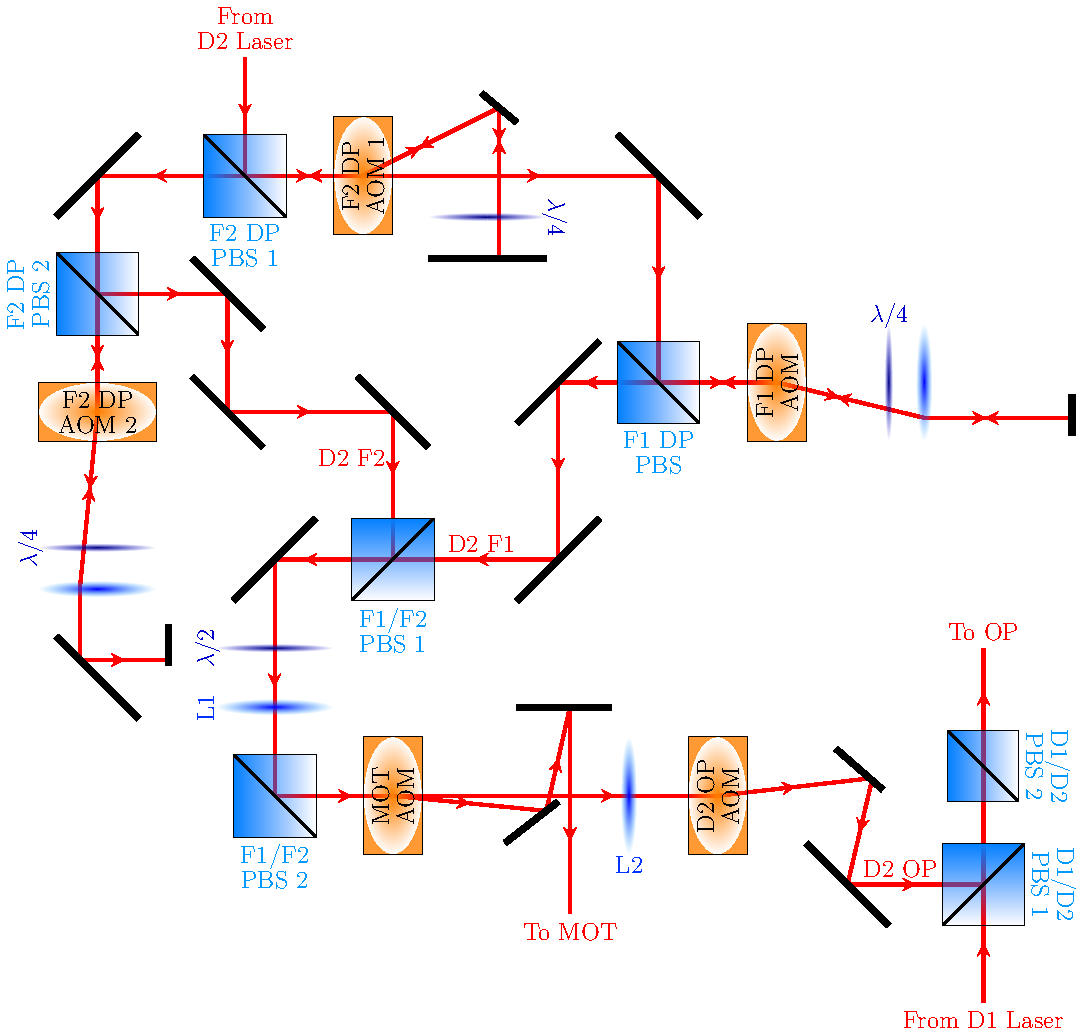
\includegraphics[width=\textwidth]{figures/loading_na_res_beampath.pdf}
  \caption[Beampath for Na D1 and D2 light.]{
    Beampath for generating the frequencies for Na MOT and optical pumping~(OP).
    (Beampath for fiber coupling and frequency locking is not shown.
    The power control for the D1 laser is also omitted.)
    The D2 laser is locked in the F1/F2 crossover line\todo{ref}.
    It is shifted down by the two F2 double-pass~(DP) AOMs to generate the frequency
    for the Na $F=2$ state and shifted up by the F1 DP AOM to address the Na $F=1$ state.
    The frequencies of the F1/F2 light are controlled by the F1 DP AOM
    and F2 DP AOM 2 respectively.
    This set up makes sure that when the F1/F2 DP AOMs are off,
    the closest frequency in the leaked light is at least detuned
    by half the F1/F2 separation~($\approx880~\mathrm{MHz}$)~\cite{steck_sodium_2019}
    and will have minimum effect on the atom.
    The F1 and F2 light are combined on F1/F2 PBS 1 and their power ratio after the
    F1/F2 PBS 2 is controlled by the half waveplate between the two PBSs.
    A similar setup is used to combine the D1 and D2 light in the OP output using
    D1/D2 PBS 1 and the rotating D1/D2 PBS 2.
    Since we need to switch the Na MOT light on and off out-of-phase
    with the Na tweezer~\cite{hutzler_eliminating_2017} at a high frequency,
    the sharpness of the turn on/off edge in the MOT AOM is important.
    We focus the beam through the AOM using lens L1 to optimize the switching time.
    This is then collimated by lens L2 for the downstream beampath.
    \label{fig:loading:free-space:na-res-beampath}}
\end{figure}

Our experiment begins with the loading of a Na Cs dual species magneto-optical trap~(MOT)
from the background pressure created by the dispensers.
It is created using six cooling beams of $\approx\todo{number}~\mathrm{mm}$ diameter
with $\approx\todo{number}~\mathrm{mW}$~(Na) and $\approx\todo{number}~\mathrm{mW}$~(Cs)
power in each beams.
The resulting MOT has a diameter of $\approx\todo{number}~\mathrm{mm}$
with $\approx\todo{number}$~(Na) and $\approx\todo{number}$~(Cs) atoms being trapped
and cooled to to a temperature of $\approx\todo{number}~\mathrm{mK}$~(Na)
and $\approx\todo{number}~\mathrm{mK}$~(Cs).
The atom numbers are significantly smaller than the ones typically seen in a bulk gas experiment
since the goal of the free-space laser cooling is to load atoms into the tweezers
which does not require large atom numbers.
The small size of the MOT requires a tigher tolerance on the MOT position
in order to overlap with the optical tweezer for the loading of single atoms,
which in turns increased the sensitivity to to the alignment
and power balance of the cooling beams that determines the MOT position.
Because of this, we use four independent fibers to deliver the power
for the four horizontal cooling beams which allows independent control
of the power and alignment.
We observed a more robust MOT and, as a result, single atom loading
compared to using retro-reflectors to create conterpropagating horizontal cooling beams.
Due to the geometric constraints in the experiment,
retro-reflector is used for verticle cooling beams.

The MOT is followed by a compressed-MOT~(CMOT) stage for Na
which uses light closer to resonant to push the Na atoms closer to the center
as well as reducing their temperature to $\approx\todo{number}~\mathrm{mK}$.
After this, the magnetic field is turned off and
a polarization gradient cooling step is applied on the atoms
which cools the atoms to $\approx\todo{number}~\mathrm{mK}$~(Na)
and $\approx\todo{number}~\mathrm{mK}$~(Cs).

The beampaths for generating all the necessary frequencies are shown in
Fig.~\ref{fig:loading:free-space:na-res-beampath}~(Na) and \todo{}~(Cs).
The same beampaths are also used for generating the light for cooling
and imaging of single atoms as well as optical pumping for state preparation
that will be discussed in later chapters.

\section{Loading and Imaging in the Tweezer}
\label{ch:loading:loading}

\todo{
  NA
  Beam path
}

\todo{
  Light shift
  Live signal
  Loading
  estimate of photon scattering number
  cite Lee's thesis
}

\section{Summary and Outlook}
\label{ch:loading:summary}

\todo{}
